\documentclass[10pt,twocolumn,letterpaper]{article}

\usepackage{dependable_dnn}
\usepackage{times}
\usepackage{epsfig}
\usepackage{graphicx}
\usepackage{amsmath}
\usepackage{amssymb}
\usepackage{subfigure}
\usepackage[table, dvipsnames]{xcolor}

% Include other packages here, before hyperref.

% If you comment hyperref and then uncomment it, you should delete
% egpaper.aux before re-running latex.  (Or just hit 'q' on the first latex
% run, let it finish, and you should be clear).
\usepackage[pagebackref=true,breaklinks=true,letterpaper=true,colorlinks,bookmarks=false]{hyperref}

\iccvfinalcopy % *** Uncomment this line for the final submission

\def\iccvPaperID{} % *** Enter the Paper ID here
\def\httilde{\mbox{\tt\raisebox{-.5ex}{\symbol{126}}}}

% Pages are numbered in submission mode, and unnumbered in camera-ready
\ificcvfinal\pagestyle{empty}\fi

\begin{document}

%%%%%%%%% TITLE - PLEASE UPDATE
\title{High-Quality Self-Supervised Deep Image Denoising\\ {\rm {\normalsize Seungmin Lee (profile2697@gmail.com; 2020-20866), \\Dept. of Electrical and Computer Engineering, Seoul National University}}}   % **** Enter the paper title and student information here

\maketitle
\thispagestyle{empty}

\section{Introduction and Motivation}
Traditional denoising methods are supervised-learning bases, requiring a pair of clean and corrupted images for each input. However, collecting such pairs is difficult and often impossible. This paper proposes a novel denoising model training method that only requires unpaired collections of corrupted images to alleviate the data collection problem. 
The proposed method predicts the clean pixel value with Bayesian reasoning based on a given noise pixel value and neighboring pixels around the noise pixel.


\section{Method}
According to the paper, all denoising methods assume that the clean pixel value $y$ depends on both the noisy pixel $x$ and the context of neighboring pixels $\Omega_x$. Concretely, they define $\Omega_x$ as pixels around the center pixel $x$ except for the center pixel.
In this kind of view, we can formulate denoising as modeling $p(y | x, \Omega_x)$. 

\subsection{Self-Supervised Bayesian Denoising}
This paper uses the following equation to modeling $p(y | x, \Omega_x)$:
\begin{align*}
	p(x | \Omega_x) = \int{p(x | y) \cdot p(y | \Omega_x)dy}
\end{align*}
where we approximate $p(x | \Omega_x)$ using training data. To approximate $p(x | y)$, the authors utilize external information in the form of an explicit model of the corruption. For example, in their experiments with additive gaussian noise, they assume that they know a given noisy image is generated by adding gaussian noise to the clean image. Moreover, the authors model $p(y | \Omega_x)$ as a multivariate guassian parameterized by $\mu_y$ and $\Sigma_y$. Approximating $p(y | \Omega_x)$ using $\mathcal{N}(\mu_y, \Sigma_y)$ also allows us to compute $(x | \Omega_x)$ in closed form.

Using the approximated $p(y | \Omega_x)$, the authors reach our denoising model $p(y | x, \Omega_x)$ using the following functional relationship:
\begin{align*}
	p(y | x, \Omega_x) \propto p(x | y) \cdot p(y | \Omega_x)
\end{align*}
Note that by assuming $p(x | y)$, we are able to model $p(y | x, \Omega_x)$ without the pairs of clean and corrupted images.


\begin{figure}[t]
	\centering
	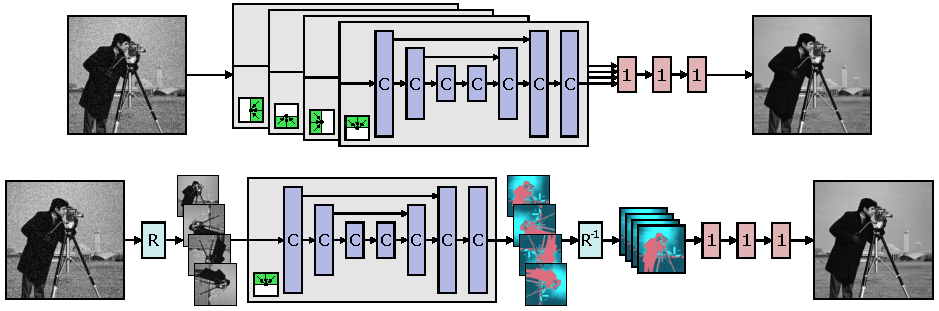
\includegraphics[width=250px]{assets/outline-3.pdf}
	\caption{(a) \textbf{Top:} In training, the network adopts four different denoising branches, and each of the branches has receptive fields restricted to another direction. (b) \textbf{Bottom:} In testing, the network uses a single branch and takes four rotated images to produce the same results with a simpler architecture.}
	\label{fig:imgs}
\end{figure}

\subsection{Convolutional blind-spot network architectures}
\label{subsec:blind}

This method calculates A, which is defined as sans the center pixel $x$, using a convolutional blind-spot network. In the training phase, the convolutional blind-spot network uses four different branches, where each branch has differently oriented blind-spot implemented as restricted receptive fields, as we can see in Figure~\ref{fig:imgs}. They implement the restricted receptive fields by masking half of the convolution kernel.
In testing, for the sake of simpler architecture, they input four rotated images to a single branch.


\section{Results}

The authors evaluate the proposed method on Gaussian, Poisson, and impulse noise. Even though the proposed method does not require supervision, the proposed method shows comparable or better performance than the existing methods. 

\section{Personal Note}
 
Although the proposed method shows comparable performance, I cannot fully agree with the assumption that we can use the explicit corruption model ($p(x | y)$). Moreover, the authors evaluate the method only on the simple noise such as Gaussian, Poisson, and impulse. Therefore, I cannot make sure the method works well on real-world noises.


% {\small
% \bibliographystyle{ieee}
% \bibliography{egbib}
% }


\end{document}
